%%%%%%%%%%%%%%%%%%%%%%%%%%%%%%%%%%%%%%%%%%%%%%%%%%%%%%%%%%%%%%%%%%%%%%%%%%%%%%%%%%%%%%%%%%%%%%%%%%%%%%%%%%%%%%%%%%%%%%%%%%%%%%%%%%%%%%%%
% This is just a template to use when submitting manuscripts to Frontiers, it is not mandatory to use frontiers.cls nor frontiers.tex  %
%%%%%%%%%%%%%%%%%%%%%%%%%%%%%%%%%%%%%%%%%%%%%%%%%%%%%%%%%%%%%%%%%%%%%%%%%%%%%%%%%%%%%%%%%%%%%%%%%%%%%%%%%%%%%%%%%%%%%%%%%%%%%%%%%%%%%%%%

\documentclass{frontiersENG} % for Engineering articles
%\documentclass{frontiersSCNS} % for Science articles
%\documentclass{frontiersMED} % for Medicine articles

\usepackage{url,lineno}
\linenumbers

\usepackage{graphicx}

% Leave a blank line between paragraphs in stead of using \\

\copyrightyear{}
\pubyear{}

\def\journal{Neuroinformatics}%%% write here for which journal %%%
\def\DOI{}
\def\articleType{Research Article}
\def\keyFont{\fontsize{8}{11}\helveticabold }
\def\firstAuthorLast{Sample {et~al.}} %use et al only if is more than 1 author
\def\Authors{Matthew McCormick\,$^{1,*}$,
  Xiaxiao Liu\,$^{1}$,
  Julien Jomier\,$^{2}$,
  Charles Marion\,$^{2}$,
  Joshua Carp\,$^{3}$,
  and Luis Ibanez\,$^1$}
% Affiliations should be keyed to the author's name with superscript numbers and be listed as follows: Laboratory, Institute, Department, Organization, City, State abbreviation (USA, Canada, Australia), and Country (without detailed address information such as city zip codes or street names).
% If one of the authors has a change of address, list the new address below the correspondence details using a superscript symbol and use the same symbol to indicate the author in the author list.
\def\Address{$^{1}$Medical Computing Group, Kitware Inc, Clifton Park, NY, USA\\
$^{2}$Medical Computing Group, Kitware Inc, Lyon, France\\
$^{3}$University of Michigan, Ann Arbor, MI, USA\\
}
% The Corresponding Author should be marked with an asterisk
% Provide the exact contact address (this time including street name and city zip code) and email of the corresponding author
\def\corrAuthor{Luis Ibanez}
\def\corrAddress{Medical Computing Group, Kitware Inc, Clifton Park, NY, USA}
\def\corrEmail{luis.ibanez@kitware.com}

% \color{FrontiersColor} Is the color used in the Journal name, in the title, and the names of the sections


\begin{document}
\onecolumn
\firstpage{1}

\title[ITK Reproducible Research]{ITK: Enabling Reproducible Research and Open Science}
\author[\firstAuthorLast ]{\Authors}
\address{}
\correspondance{}
\extraAuth{}% If there are more than 1 additional author, comment this line and uncomment the next one
%\extraAuth{corresponding Author2 \\ Laboratory X2, Institute X2, Department X2, Organization X2, Street X2, City X2 , State XX2 (only USA, Canada and Australia), Zip Code2, X2 Country X2, email2@uni2.edu}
\topic{Research Topic}

\maketitle
\begin{abstract}

\section{}
%As a primary goal, the abstract should render the general significance and conceptual advance of the work clearly accessible to a broad readership. References should not be cited in the abstract.
%See the Summary Table at \\ \url{http://www.frontiersin.org/}\texttt{\journal}\url{/authorguidelines} \\for abstract requirement and length according to article type.
The essential feature of the scientific method is the practice of verification of reproducibility.The large majority of research activity today is focused on generating novelty, and only in exceptional cases, concerned with the verification of reproducibility. The practice of peer-review has been assumed to be a suitable replacement for the verification of reproducibility, a mistake by which experimental work has been replaced by thought experiments and opinion-based evaluations that do little to further the scientific enterprise. This drift has denigrated, what used to be scientific work, back into the practice of the “natural philosophy” in which we simply imagine models of the natural word and evaluate them based on aesthetic appeals and desire for self-consistency.

The Insight Toolkit (ITK) has made it possible to restore the true practice of the scientific method in the field of medical image analysis. By providing a common platform in which image analysis algorithms and processing techniques can be implemented and can be freely disseminated. ITK empowers all to verify the experimental work of image analysis research activities. This of course, requires that researchers adhere to the true practice of the scientific method and publish the full details of their methodology, including the source code, data, parameters and auxiliary documents that are required for a third party to independently repeat the work and verify the findings.

The ITK community created in 2005 a scientific journal, the Insight Journal, truly fulfilling the practice of the scientific method, where all articles are required to provide the full set of source code, data and parameters needed to reproduce the finding of the authors. These materials are immediately made available to readers and reviewers, empowering them to indeed perform such verification with minimal effort and minimal loss of information.

Other Journals, in particular Frontiers, PLoS, and more recently Nature, have embraced this restoration of the true practice of the scientific method.  With the support of the Reproducible Research movement, these progressive publication venues are creating the conditions for a new age of enlightenment in which the methodologies of practical research work will not be subject to secrecy, nor be subject to the veil of suspicion that many incidents of scientific fraud and data manufacturing that have left us with in recent months.

The open source nature of ITK, the open access nature of the Insight Journal, and the public sharing of open data that is enabled by the Midas Platform in the ITK community, are the three pillars of Open Science that are transforming the way scientific research is done today.

The technological challenges of reproducibility have all been solved. We now require a cultural change by which we must make simply unacceptable that any article in the domain of medical image analysis be published without the full set of source code, data and parameters that will enable an independent group to replicate the process and verify or refute the findings.


\tiny
 \keyFont{ \section{Keywords:} Reproducibilty, ITK,Insight Journal, Code Review, Open Science} %All article types: you may provide up to 8 keywords; at least 5 are mandatory.
\end{abstract}


\section{Introduction}

% For Original Research Articles, Clinical Trial Articles, and Technology Reports the introduction should be succinct, with no subheadings.
%
%For Clinical Case Studies the Introduction should include symptoms at
%presentation, physical exams and lab results.
%
The National Library of Medicine’s Insight Segmentation and Registration
Toolkit (ITK) was conceived in 1999 to support analysis of The Visible Human
Project data. In order to maximize its impact, the project embraced an open
source development model from its inception. Not only was the project
successful in its original objective, it also extended far beyond its original
goals and became a foundational component of many National Institutes of Health
(NIH) research projects, as well as evolved into a technology underlying many
medical image analysis commercial products worldwide.

%
%The following numbers were computed with the script:
%src/git-lines-of-code-statistics.sh
%
The ITK repository currently contains over 2.5 million lines of source code
(including 1.2 million lines of third-party code added to the repository).
Contributions to this repository can be measured by the number of logical
changes made to the code, also known as commits, and the number of source code
line additions or deletions. In its 14 years of history, ITK has received
37,626 commits, in 13,184 files, by 209 different authors.

Ohloh.net \cite{OhlohITK2013} is a public directory of open source projects that performs analytics on the code history of communities surrounding projects. According to its
Project Cost Calculator, the effort in the toolkit is an
estimated 730 person-years, amounting to an estimated cost of 40 million
dollars given an average salary of \$55,000 per year.

As of October 29, 2013, the combined subscribers to the \textit{community},
\textit{insight-users}, and \textit{insight-developers} mailing lists are 2,698.
The lists average 326 messages per month from October 2012 to October 2013.


\section{Material \& Methods}

\subsection{Software Quality Assurance}

To ensure the code quality of the toolkit and the growth of the community,
adaptation to modern software practices are necessary. In particular, the
recent modernization of ITK includes a version control system (Git) , a code
review system (Gerrit), a Gerrit-integrated dashboard testing system
(CDash@Home) and modularization.

\subsubsection{Source Code Version Control: Git} Git is an open source
distributed version control system designed to perform with speed and
efficiency. It features with cheap local branching, convenient staging areas,
and multiple workflows, which are particually useful for large open source
projects like ITK. When migrating the source code repository from CVS to Git,
we managed to preserve the entire ten year history of the project, and  a Git
workflow was customized for the pracices of the ITK developers.

The adoption of Git empowered ITK developers to easily create flexible
workflows of branching and merging. It also allows developers to
make commits even when they are not connected to the network. Despite the
initial learning curve to master several commonly used git commands, Git creates
a superior collaboration platform for the commumity.  It also make it possible
to embrace the most popular open source code repository site GitHub and adopt
the code review system: Gerrit.


\subsubsection{Open Review System: Gerrit Review} In the context of
reproducible science, the detailed description of the methods and materials
used to perform an experiment are a fundamental piece of the article that
disseminates the results. As research activities become more and more dependent
on software for the preparation, execution and analysis of experiments, it
becomes necessary to include all the details related to the software as part of
a reproducible publication. Given the complexities of software implementation,
mere algorithmic descriptions, or even pseudo-code are not sufficient to ensure
reproducibility through reimplementation. Only the delivery of original source
code can provide enough assurances that the recipient of the materials will be
able to replicate the reported work with a reasonable limited amount of effort.

The code must therefore be subject to peer review processes similar to the ones
currently used for scientific publications. Such reviews should examine both
the quality and correctness of the code, as well as proceed to verify the
reproducibility of the code through its execution.

Recently, recognition of software’s importance for the progress of science has
elicited movements such as the Science Code Manifesto \cite{Barnes2010}. While
a number of journals are beginning to adopt practices similar to The Insight
Journal, where code is submitted along with the article, evaluation tools and
procedures for peer review of the code are not in parity with those used for
the article.  Commonplace practices have evolved to facilitate article review
such as evaluation rubrics, instrumentation of the text with line and page
numbers for reference during discussion, and a process to distribute an article
to reviewers and communicate author replies.  While this provides the reviewers
with a mechanism to evaluate the reproducibility, and therefore the merit, of
the article, the technical nature of code solicits greater technical
capabilities of the tools and methods used to evaluate its reproducibility.

While this problem is multi-faceted, some progress has been made through ITK’s
adoption of the Gerrit Code Review system.  Gerrit is an open source project
maintained by the Google Android mobile phone project. This systems enables a
large community of developers to inspect and comment on the code changes that
are proposed for inclusion in a software system. Not only has the ITK community
embraced the use of Gerrit, it has also contributed fixes and features back to
the Gerrit project.

Gerrit is implemented as a combination of a web-based front end with a Git
repository backend. Most of the interactions that developers have with Gerrit,
happen with the web-based front end server. The Gerrit server provides a
mechanism to effectively evaluate code changes, obtain and test those changes
locally, and perform notification and transmission of the changes and comments
for authors and reviewers, as well as management of the system to accept
merges.

Gerrit is a technology that is built around the Git distributed version control
system.  With Git, contributors can independently develop and test patches that
are put in topic branches created out of the ITK master branch.  Next, the
patch can be shared with the community by pushing the topic branch to the
Gerrit server \cite{ITKGerrit}.  Once in the server, the change is publicly
accessible via the web-based front end.  Developers can then use a web-browser
to see side-by-side differences that are easily identified with
color-highlighting, on a file-based diff page.

From the web interface, contributors can request the attention of specific
reviewers to comment on their patch. As a convenience, the web-interface
provides auto-completion of names for any community member that has registered
an account with the server.  The reviewers for a given change can be added or
removed throughout the review process by any community members, and they will
be notified via email of any new comments or change revisions.  In the Gerrit
system, every change is identified by a unique Change Id, which allows multiple
revisions, also known as Patch Sets, to be uploaded consistently in response to
comments.

The discussion of the change between author and reviewers occurs via three
mechanisms: overall comments on the change, inline comments, and numerical
ratings. Overall comments conveying general remarks can be added per Patch
Set, and the history of comments is retained and easily navigated. Questions
and suggestions can be directed at specific sections of the code with the
inline comments. Whether the code can reproducibly be built and pass tests is
indicated by the reviewer with a numerical Verified score, and overall
evaluation is indicated with a numerical Code Review score. With the Gerrit
Code Review system, reproducibility is improved through continual refinement of
the corpus of Insight Toolkit knowledge, as embodied in the code repository,
through experimentation as implemented in the unit tests, and through peer
review as exercised in the code reviews.

\subsubsection{Open Dashboard} ITK has a stringent system of quality control
that uses a combination of unit testing, regression testing, multi-platform
verification, and continuous integration. The testing infrastructure of ITK
includes more than 2,400 unit tests, which provide a code coverage of 84\% of
ITK code lines. This is well above the industry averages of 50\% code coverage.

The collection of unit tests are executed nightly by computers contributed by
community members all around the world, and reporting to a central online
dashboard that summarizes the results. This web-based dashboard system (CDash)
\cite{ITK dashboard} ensures ITK’s software quality as developers around the
world continuously make changes to the code base. Build status and regression
test status are visualized in a tabular form. The dashboard is an important
coordination and communication tool that empowers developers to share the
results of a local test with other developers by pushing them to the online
summary pages.

Continuous builds triggered by patches submitted to the Gerrit code review
system also give feedback to developers on the impact of recent changes.
Nightly builds of the project spanning a wide variety of platforms and
configurations ensure that ITK can be built on a diversity of operating systems
and hardware.



\subsection{Sustainability}

\subsubsection{Community Enablement}

In particular, we have successfully hosted a series of webinars to promote ITK
and the new features available in ITKv4. The webinar videos received more than
1,000 plays in total. We have begun moving to hosting more advanced topics,
such as “Raspberry Pi Likes ITK” and “Raspberry Pi Likes ITK with VTK”. To
empower new developers and lower the barrier of entry for new users, we have
initiated a web framework to better distribute ITK examples and put together a
large collection of examples on various ITK classes and filters.

In a very focused effort to grow the ITK community, an online space called
ITKBarCamp was created to train new community members on the software
technologies that are essential to ITK. This space provides a combination of
source code, documentation and video tutorials that guide newcomers at their
own pace through training materials aimed at honing their software development
skills.

One of the very active areas in the ITK BarCamp is a series of participatory,
short YouTube.com videos with associated documentation covering various topics
related to ITK, including: \begin{enumeruate} \item Mastery of the command line
\item Basic C++ programming skills \item Good software practices, including
unit testing \item Recommended tools and workflows for ITK development.
\end{enumerate}

So far we have created 29 short tutorial videos, which have received 2,234
views and attracted 30 subscribers. ITK Bar Camp materials are hosted in Github
as written documentation and video archives. Information on previous and
current webinars and hangouts can be found at
http://www.itk.org/ITK/resources/webinars.html.

We believe these efforts are crucial to attracting, training, and retaining new
community members in the long run, and through that mechanism replenish the
community with active members. We plan to continue collecting bar camp
tutorials and encourage other community members to contribute to the
repository.

\subsubsection{Modularization} Since its inception in 2000, ITK was designed as
a collection of about seven core libraries and about ten third party libraries.
This monolithic organization of the code over time led to very large
sub-libraries as more classes were added to the toolkit. Once the core code of
ITK surpassed the half-a-million lines of code, it became evident that a more
modular approach was needed in order to support the future continued growth of
the toolkit.

\textbf{Figure 1.}{An illustration on ITK modules' dependencies.}\label{fig:01}

As a result of the modularization, the initial monolithic code base of about
12,000 files was partitioned into more than 100 modules.  And as of Oct of
2013, ITK contains 141 modules in total, four of which are remote modules
\cite{remote modules}.  Dependencies \ref{fig:01} between modules were
identified and explicitly declared in the CMake-based configuration system. By
making the CMake-based configuration system aware of the new ITK
modularization, the modularization empowers ITK adopters to select the pieces
of ITK that they wanted to use in their own projects at configuration time.
Support for integrating externally distributed modules was built into the
modularization infrastructure.The Remote Module infrastructure enables fast
dissemination of research code through ITK without increasing the size of the
main repository.


\subsection{Open Publication: The Insight Journal}

ITK has been conceived as a usable encyclopedia of image analysis algorithms
that are of particular utility to the medical imaging community. Given the
rapid pace at which technology develops in this area, and the proliferation of
both generic and specialized image analysis algorithms, it is important for ITK
and its community to continuously update the content of the toolkit by adding
new algorithms while simultaneously improving and extending existing ones. To
do this, the ITK community relies on contributions made by its members, as they
use the toolkit to support their own projects and run into situations where
additions and improvement are required for them to achieve their goals. In
order to absorb these contributions, the ITK community has used the Insight
Journal \cite{Insight Journal} }since 2005. The online Insight Journal
publishes practical articles written by developers for developers, and requires
those articles to be fully reproducible.

The Insight Journal is a free, open-access publication covering the domain of
medical image processing and visualization.It enables community members to
publish their contributions to medical projects for open peer-review, full
reproducibility verification, and open-rating by readers worldwide.

The journal is very active, and since its inception in 2005, it has published
542 articles with 826 public reviews and has more than 2,500 subscribed
readers. The top four articles have been downloaded more than 5,000 times and
viewed more than 10,000 times. The Insight Journal is currently the only
technical publication in the domain of image analysis that not only allows but
also requires verification of reproducibility as part of the submission and
review process. The importance of restoring the practice of reproducibility
verification in scientific research has resurged in recent years in light of
worrisome findings of inconsistency, lack of quality and even fraud in what
were otherwise considered to be high-quality publications. By adhering to a
reproducibility verification requirement, the Insight Journal ensures that
community members get rapid access to reliable publications that include open
source software that they can readily use in their projects.

Insight Journal now accepts ITK module submissions. This feature empowers
community members to take advantage of the new modular structure in ITK and
makes future code integration easier. Readers can then download Insight Journal
articles and directly plug-them-in as modules of their local ITK installation.


\section{Results}

Contribution Statistics
\subsection{Software Quality Assurance}

\subsection{Open Review System: Gerrit Review}
In the three years that the community has applied the Gerrit Code review
system, << d['src/gerrit_results.json'].from_json()['changes'] >> changes have
been submitted to the review server and
<< d['src/gerrit_results.json'].from_json()['reviews'] >> were performed.
As a matter of policy, all merged changes should have at least one review,
but the number of iterations on a change varies flexibly depending on the
requirements. This results in a roughly negative exponential distribution in
revisions, as evident in the histogram of revisions in
Figure~\ref{fig:gerrit_patch_set_histogram}.  The highest number of reviews
for a single change was
<< d['src/gerrit_results.json'].from_json()['max_reviews'] >>.

Two direct but notable conclusions follow from this data. First, at least one
other person examined and reproduced a proposed code.  This certainly exceeds
publication systems where the code is never dissemminated, and it likely
exceeds validation systems where the code is published, but there are not
incentives or checks that reviewers looked at or applied the code.

The number of Patch Sets greater than one also implicitly indicates that
improvements were made and errors were identified by this process.  This is
hypothesis is further supported by Figure~\ref{fig:gerrit_fix_ups}.  In this
figure, the number of "fix-up" changes are quantified. A fix-up change is
defined in an objective way that roughly captures changes that were likely
intended to correct or improve a recent defect that was introduced.  Sections
of a patch, traditionally called hunks, that are additions or modification are
identified, and all commits in the following five days are examined.  If
content in the committed hunk is modified in that period, it is labelled as
fix-up commit.  If addition or modification hunks in the fix-up commit are again
modified in the following five days, then the original change is said to have
two fix-up commits, and so on.

We computed fix-up commits in the ITK repository for a three year period
preceeding the adoption of the peer code review system from August 25th, 2007
to August 25th, 2010 to the three year period following from August 25th, 2010
to August 25th, 2013.  There were
<< d['src/gerrit_results.json'].from_json()['pre_gerrit_commits'] >>
changes during the pre-peer code review period and
<< d['src/gerrit_results.json'].from_json()['post_gerrit_commits'] >>
during the post-peer code review period.  As shown in
Figure~\ref{fig:gerrit_fix_ups}, this reduces the number of
single fix-up commits from <<
d['src/fix_up_bins.json'].from_json()['single_pre'] >>\%
to << d['src/fix_up_bins.json'].from_json()['single_post'] >>\% and
dramatically reduces the percent fix-up commits by approximately half for
higher numbers.

The underlying cause of this apparent reduction in errors is suggested by the
graph visualization of Figure~\ref{}. This graph sources the three years of
reviews performed by the Insight Toolkit community. Each node is a community
member, and the size of the node is logarithmically related to the accumulated
number of changes created by that community member.  The edges in the directed
graph represent accumulated reviews given by one community to another. A
number of high level observations can be made from this graph.  First, there
is a spectrum of node sizes and connectivities that correspond to varying
degrees of contribution. While there are some node pairs that have mutually
strong connections, the reviews are generally well distributed.

Insight Journal
* Number of Submissions
** Number of Revisions
* Number of Reviews
* Integration into the main repository


\section{Discussion}
Software Quality assurance
The code review system helps catch bugs, results in design improvements, assists in the training of new developers, and provides a great communication platform for collaborative development. Since it has so many software quality advantages, code reviews are as critical to ITK as the creation of new patches.


Insight Journal
Past barriers from getting from the Insight Journal into the Toolkit.  Opinions on the
non-blinded review effectiveness.

The review graph indicates there is not a binary distribution of "users" and
"developers", but there a continuous transition in contribution and experience
by community members. There are not a few single nodes from which radiate all
knowledge and advancement, but a bi-directional network where knowledge and
experience can flow thoroughly.  Indeed, all the large nodes have many
incoming edges. The graph is also not grouped into islands of
isolated knowledge, but it is fully connected with few hops from any given
community member to another community member.

These properties are the result of policies and practices that encourage their
emergence. Firstly, the adoption of the Gerrit Code Review tool places an
explicit emphasis on code review.  Registration for an account is publically
without any permissions required, and the default permissions allow community
members to not only submit changes but also perform reviews. All community
members, including the novice ones, are also highly encouraged to perform
reviews in project documenation, which promotes the culture of open code
review. Second, the policy of requiring a positive code review, even for the
most experienced community members, encourages continuous improvement of even
senior members while promoting civility. It discourages obstructionism and
encourages collaboration by promoting reciprocal constructive criticism.



\section*{Acknowledgement}
Thank NLM, ITK community


\paragraph{Funding\textcolon} The US National Institutes of Health National Library of Medicine (NIH-NLM) has been a primary funder of the Toolkit since its inception 14 years and currently supports the work of authors Ibanez, Liu, and McCormick.




%----- all the figures ----------------
\begin{figure}
  \centering
    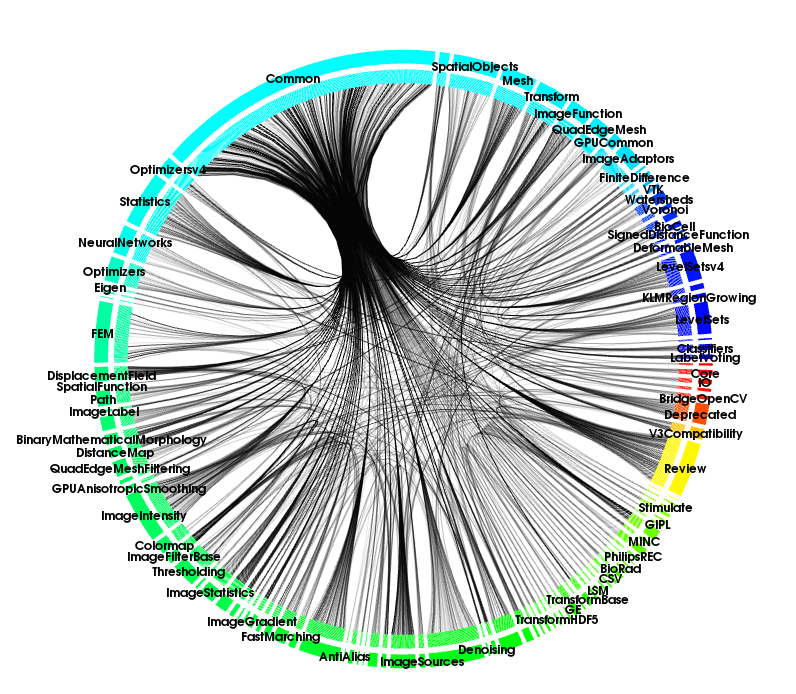
\includegraphics[width=0.5\textwidth]{itk_module_dependency.png}
    \caption{An illustration on ITK modules' dependencies.}
    \label{fig:itk_module_dependency}
\end{figure}

\begin{figure}
  \centering
    \includegraphics[width=0.5\textwidth]{gerrit_patch_set_histogram.eps}
    \caption{Histogram of the number of revisions (Patch Sets) for a given change.}
    \label{fig:gerrit_patch_set_histogram}
\end{figure}

\begin{figure}
  \centering
    \includegraphics[width=0.5\textwidth]{gerrit_fix_ups.eps}
    \caption{Fix-up commit percentage before and after peer code review.}
    \label{fig:gerrit_fix_ups}
\end{figure}

\begin{figure}
  \centering
    \showthe\textwidth
    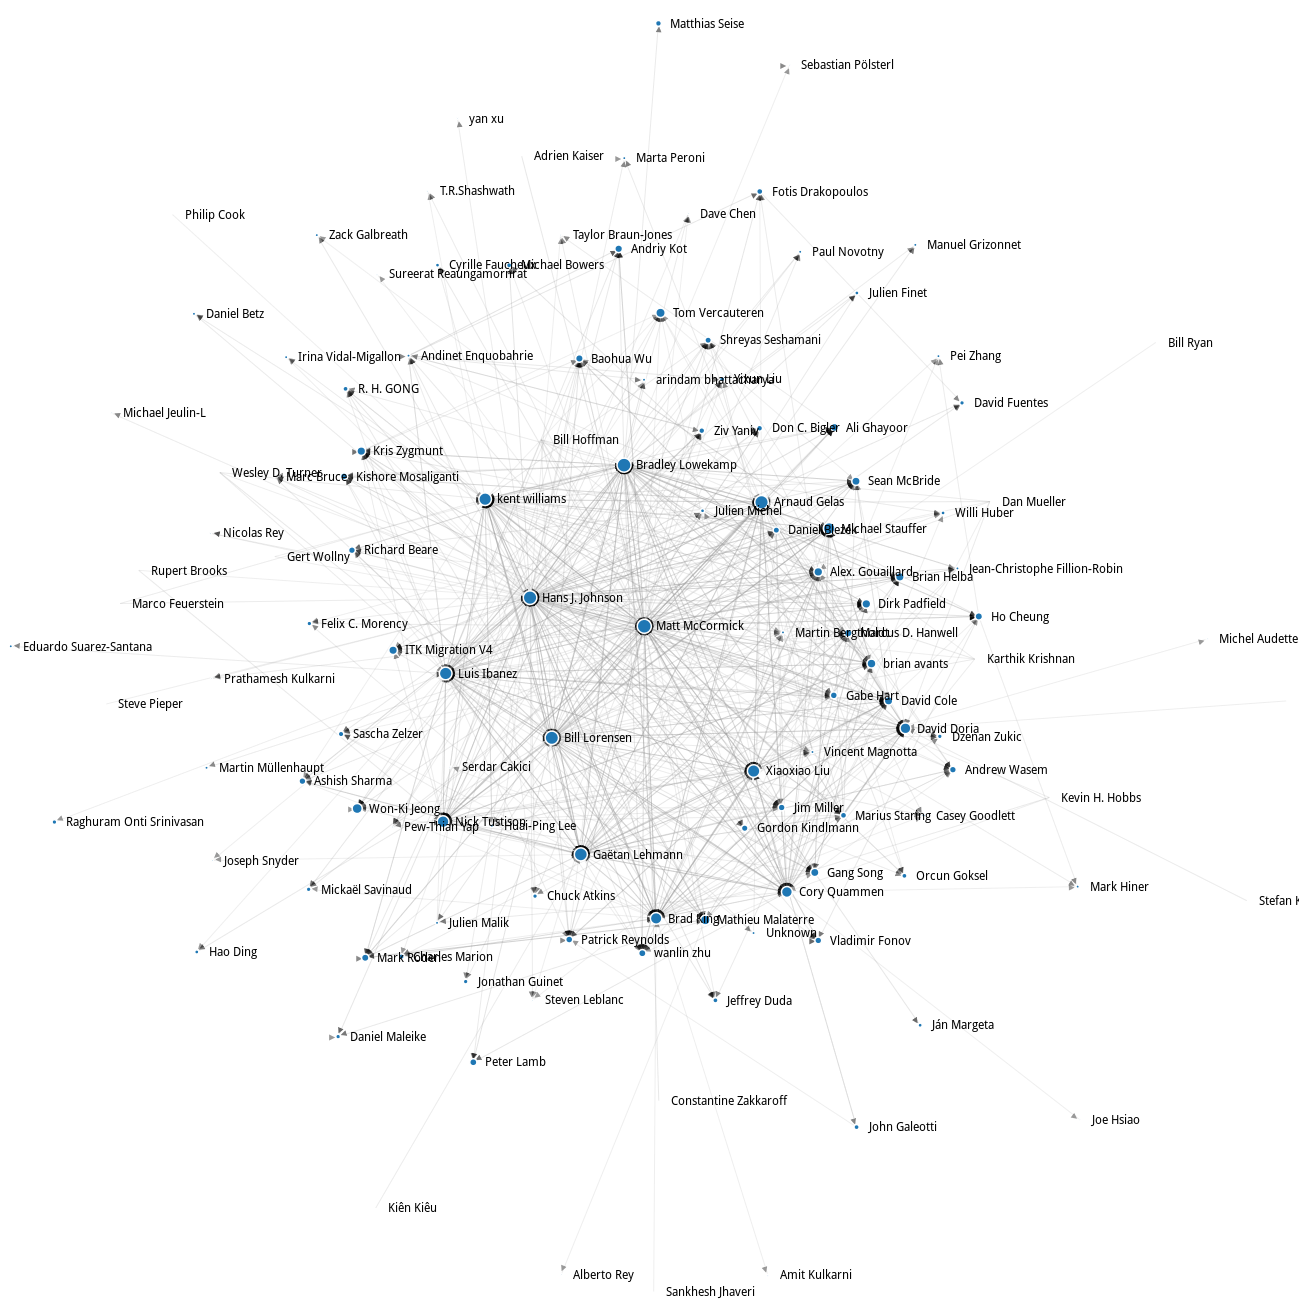
\includegraphics[width=1.0\textwidth]{GerritGraphRender.png}
    \caption{Peer code reviews graph.  Nodes are individual community members and
      size of the circle at the node is related logarithmically to the number of changes
      created by that community member.  The widths of the edges in this directed
      graph are logarithmically proportional to the number of reviews performed.}
    \label{fig:gerrit_graph}
\end{figure}

\begin{figure}
  \centering
    \includegraphics[width=1.0\textwidth]{gerrit_closeness.eps}
    \caption{Normalized closeness centrality of peer code review graph versus
      the number of created changes.  Different connected components are shown
      in different colors.}
    \label{fig:gerrit_closeness}
\end{figure}




\bibliography{frontiers}
\bibliographystyle{frontiersinSCNS&ENG} % for Science and Engineering articles


\end{document}
